\chapter{Projeto Conceitual}
\section{Geometria Interna}
Com base nos parâmetros levantados na seção anterior e em requisitos normativos aplicáveis, procedeu-se ao dimensionamento detalhado da geometria interna da cabine. Conforme observa Raymer (1992), o arranjo interno de uma aeronave é ditado mais por decisões de mercado do que por regulamentações, fato que se reflete diretamente na padronização de pitch, largura do assento e largura do corredor observada entre as aeronaves previamente estudadas.

Nesse contexto, a configuração aqui apresentada corresponde à configuração comercial para transporte de passageiros, identificada pelo estudo de mercado como a operação predominante ao longo da vida útil de aeronaves similares. A configuração cargueiro, que utiliza os mesmos trilhos estruturais para receber Unit Load Devices (ULDs), contêineres e pallets padronizados, será abordada em seção posterior.

Conforme discutido anteriormente, a cabine adotará uma configuração de 4 assentos por fileira, separados por um corredor central - padrão dominante na classe de turboélices regionais desse porte. Para escolha das dimensões internas, utilizou-se como referência principal a Tabela 9.1 de Raymer (1992), que fornece valores típicos de pitch, largura de assento, largura e altura de corredor, e volume de galley para as categorias de primeira classe, econômica e alta densidade.

A aeronave projetada enquadra-se predominantemente na categoria econômica, com elementos da coluna de alta densidade em função da faixa de capacidade especificada na descrição da missão (60 a 70 PAX) e do caráter regional de curto e médio alcance da missão.

O comprimento da cabine foi definido em 16.00 m, correspondente à média dos valores observados em aeronaves do estudo comparativo. Além disso, esse valor se mostrou adequado para acomodar a capacidade proposta de passageiros e está próximo ao da aeronave de referência mais similar - o ATR-72 (17.00 m). A largura da cabine foi definida em 2.6 m, valor também coerente com aeronaves similares e adequado para comportar os assentos e o espaço de corredor desejado. O layout em planta resultante é apresentado na Figura~\ref{fig:layout_planta}.

\begin{figure}[H]
\centering
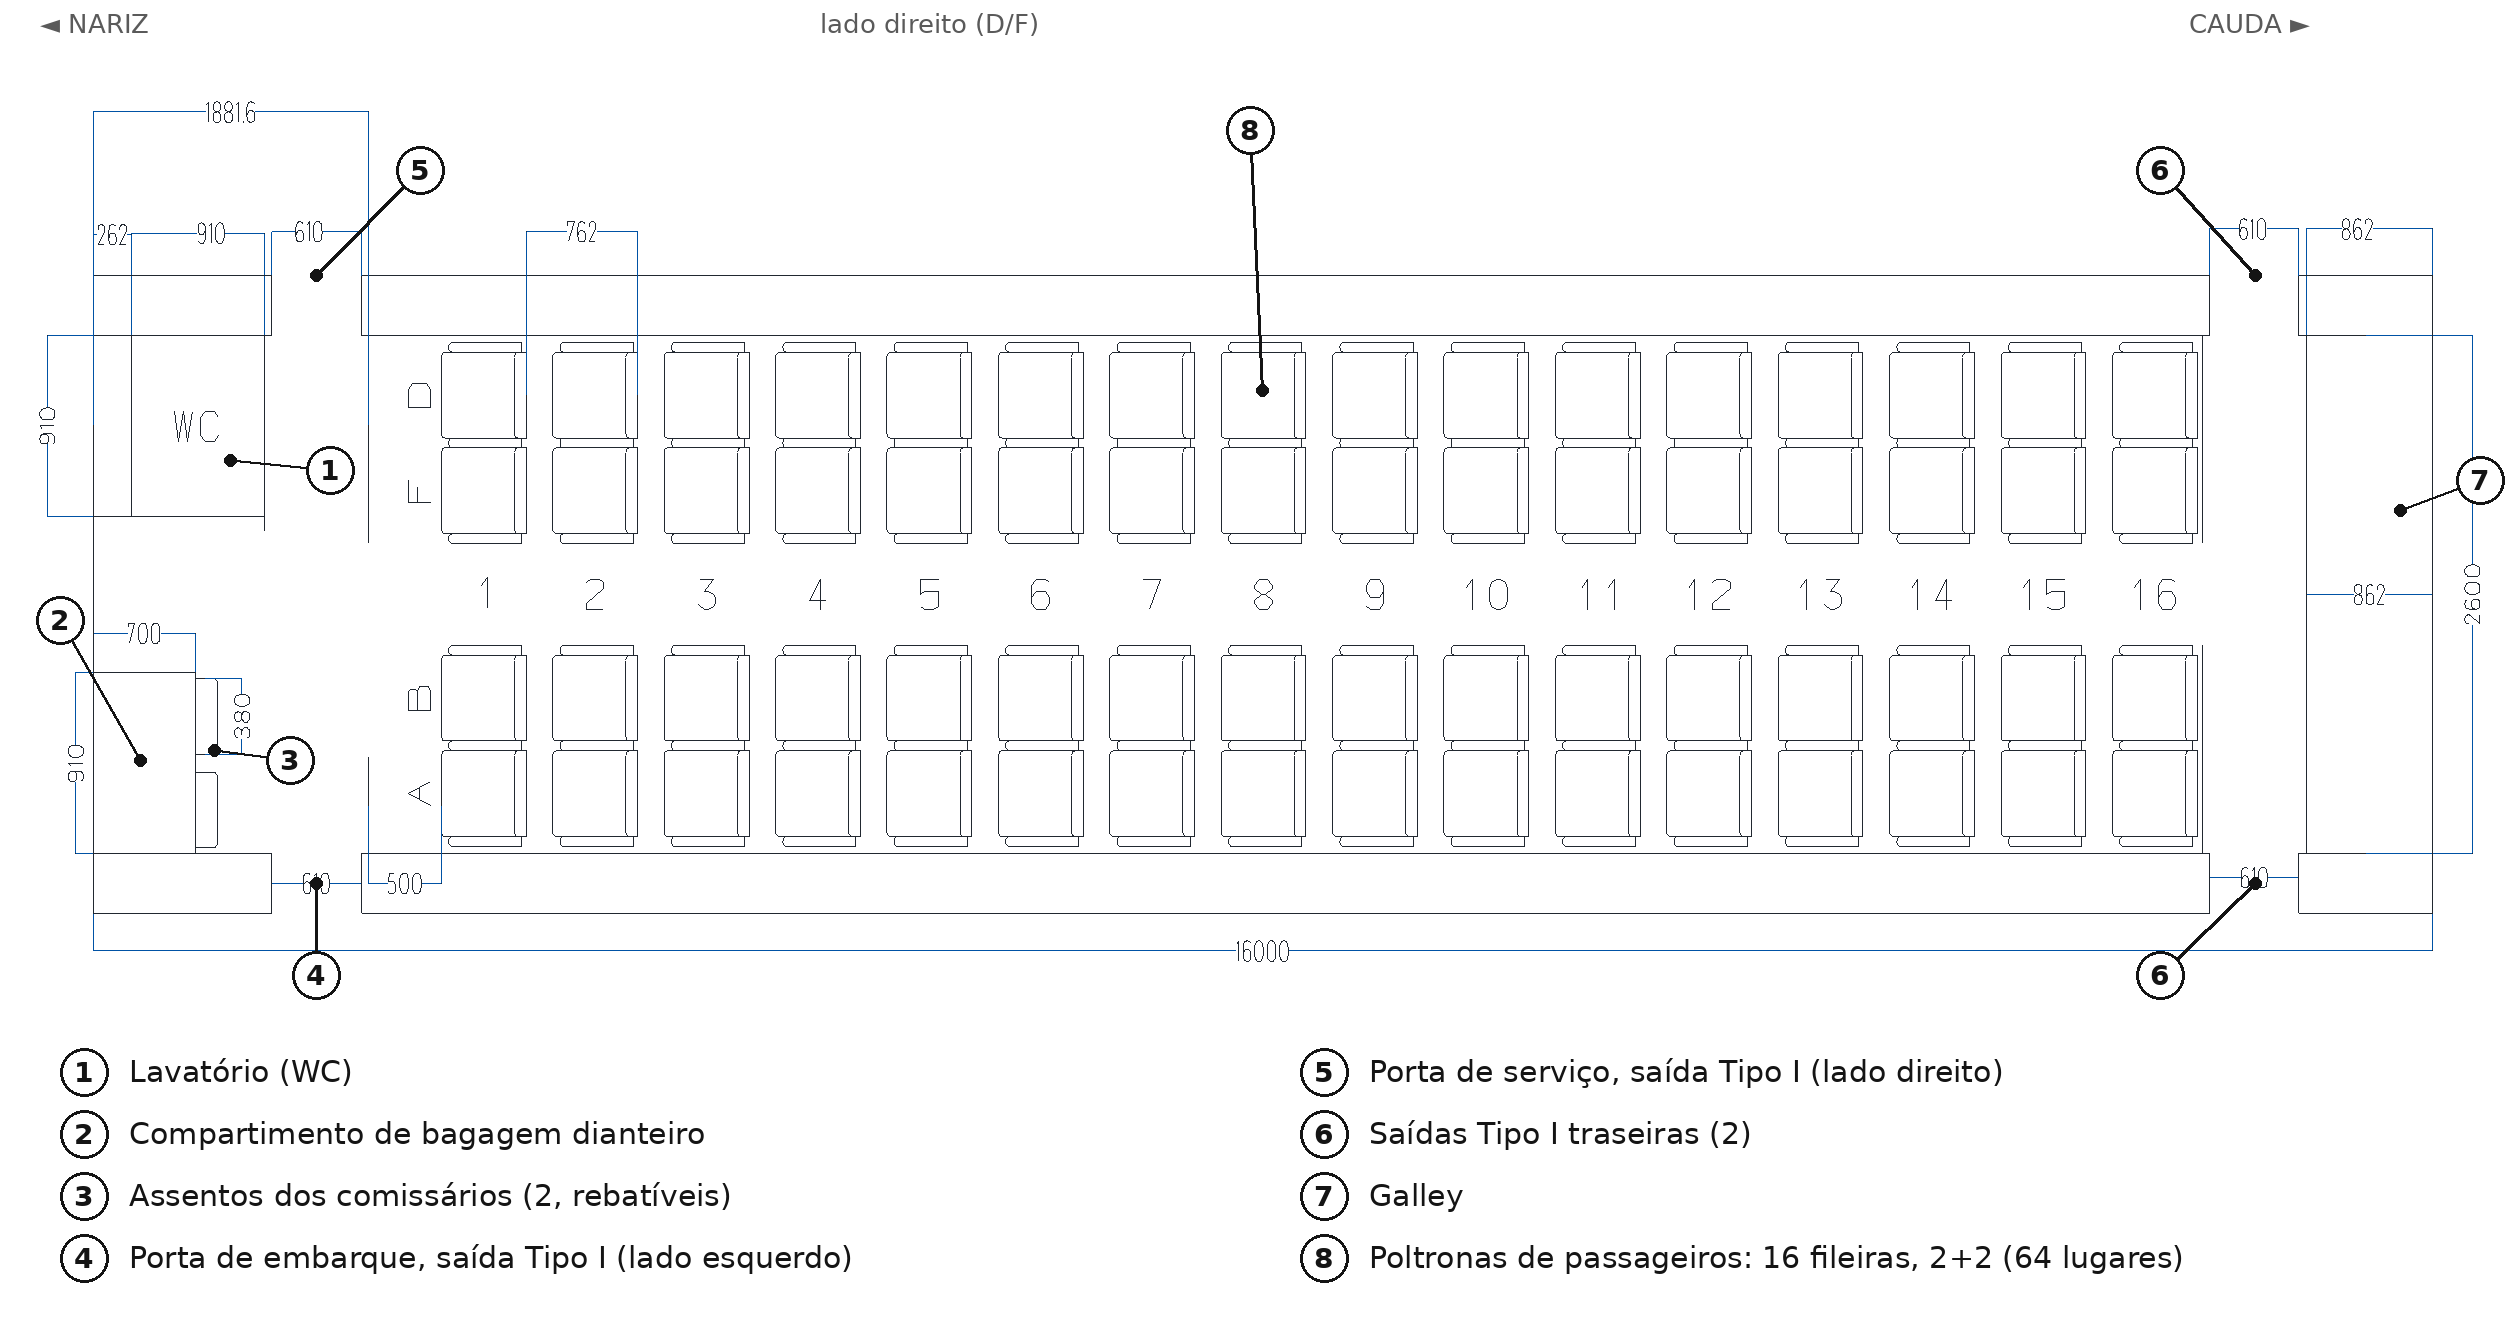
\includegraphics[width=\textwidth]{images/cabine_planta.png}
\caption{Layout em planta da cabine de passageiros, com indicação dos assentos dos comissários, saídas, lavatório, galley e compartimento de bagagem. Dimensões em milímetros.}
\label{fig:layout_cabine}
\end{figure}

Conforme mostra a figura, a cabine comporta 16 fileiras numeradas de 1 a 16, com identificação pelas letras A/B (esquerda) e D/F (direita). O pitch adotado é 762 mm (30 in), enquadrando-se na faixa de 30 a 32 in da categoria de alta densidade indicada por Raymer (1992). Nas extremidades da cabine, a zona de serviço dianteira ocupa 1881.6 mm de comprimento, acomodando um lavatório, dois compartimentos para pequenas bagagens, duas saídas de emergência (incluindo a porta de embarque) e dois assentos para tripulação. O lavatório foi posicionado na zona dianteira de modo a facilitar o acesso pela tripulação quando aplicada a configuração de carga. A zona de serviço traseira compreende 1625.5 mm de comprimento, compreendendo a galley e duas saídas de emergência. A capacidade total resultante é de 64 passageiros.

No que se refere às saídas de emergência, o RBAC 25.807 exige que todos os ocupantes possam evacuar a aeronave em até 90 segundos. Então, o layout prevê quatro saídas de emergência Tipo I posicionadas nas zonas dianteira e traseira (largura mínima de 610~mm, altura mínima de 1220~mm). Essa combinação de saídas atende plenamente ao requisito normativo de capacidade de evacuação e está coerente com as aeronaves analisadas, garantindo fluxo suficiente mesmo na condição de máxima ocupação prevista.

Ainda com base no comparativo previamente apresentado, também foi feito o dimensionamento detalhado da seção transversal, apresentada na Figura~\ref{fig:secao_transversal}.

\begin{figure}[H]
    \centering
    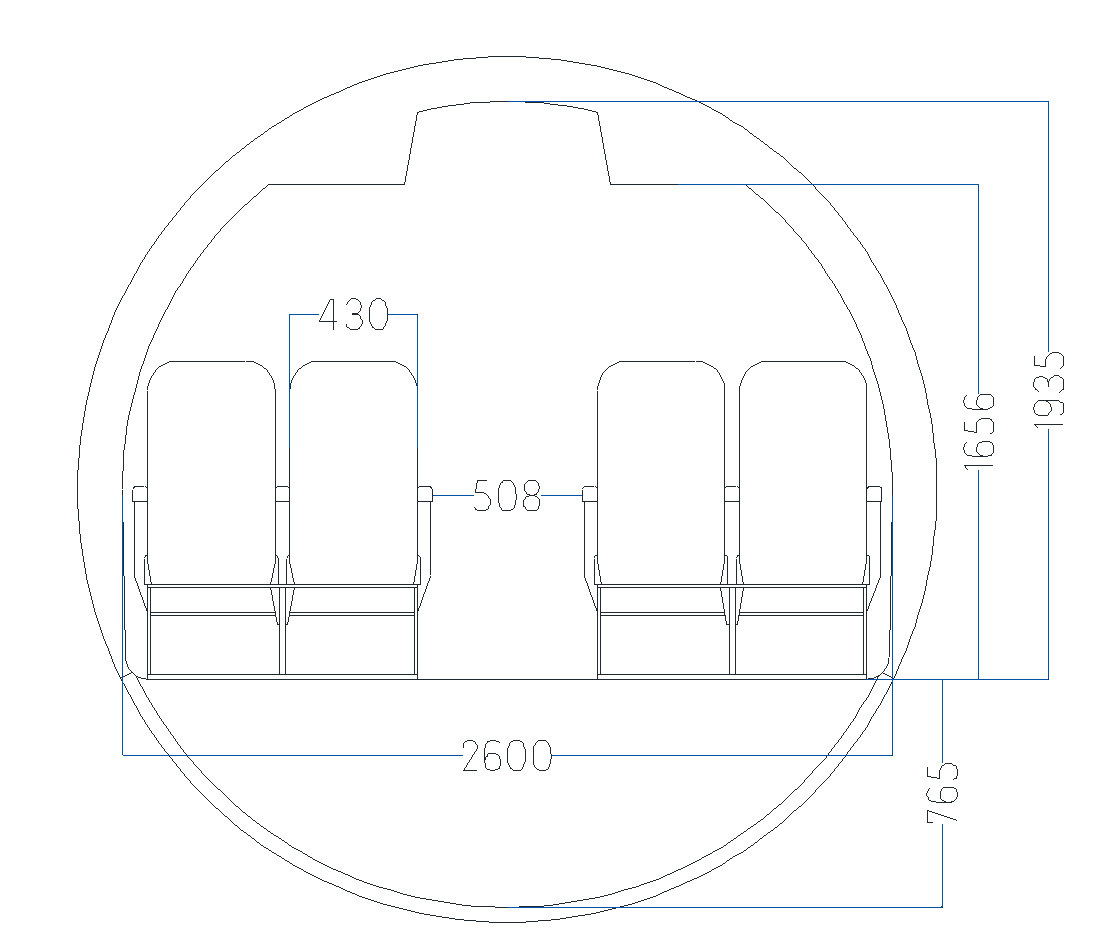
\includegraphics[width=0.65\linewidth]{images/secao_transversal.png}
    \caption{Seção transversal da cabine com configuração 2+2. Dimensões em milímetros.}
    \label{fig:secao_transversal}
\end{figure}

Cada assento possui 430 mm (16.9 in) de largura, valor compatível com a faixa de 16 - 22 in proposta por Raymer (1992) para as categorias econômica e alta densidade. O corredor central foi dimensionado em 508 mm (20 in), também enquadrando-se na faixa proposta e superando os limites mínimos de 381 mm ao nível do ombro e 406 mm ao nível do quadril estabelecidos pelo \S 25.815 do 14 CFR Part 25. As dimensões de encosto de braço e suportes dos bancos foram estimadas com base em imagens de aeronaves similares.

A altura livre interna, medida do piso até o teto sobre o corredor, é de 1935 mm (76.2 in), consistente com aeronaves similares e com o limite mínimo de 76 in indicado por Raymer (1992) para as categorias econômica e primeira classe, e consistente
com as aeronaves do comparativo. A altura entre o piso e compartimento superior (overhead bin) é de 1656 mm (65.2 in), também compatível com a categoria de primeira classe e econômica. A cota de 765 mm entre o piso e a base da estrutura engloba o assoalho estrutural, os trilhos de fixação de assentos e a câmara inferior destinada ao porão de carga.

Complementando a versatilidade operacional da aeronave, projetou-se uma configuração de carga do tipo \textit{Quick Change} (QC), que permite a conversão da cabine de passageiros para cargueiro em tempo reduzido. Esta flexibilidade é fundamental para a operação regional, permitindo que a aeronave atenda ao transporte de passageiros em horários de pico e atue como cargueiro puro em períodos de baixa demanda ou voos noturnos.


Para a operação cargueira, selecionou-se o palete padronizado IATA PLA (Half Pallet), com dimensões de base de $1534 \times 3175$ mm, conforme a figura \ref{fig:palete} em anexo. A escolha deste dispositivo justifica-se pela total compatibilidade com a infraestrutura logística global, facilitando a intermodalidade. 


Embora a cabine possua um diâmetro interno de 2,6 m, o uso do palete PLA permite a manutenção de um corredor funcional para inspeção ou folga estrutural de $0{,}53$~m. Diferente de contêineres rígidos, o palete com rede oferece a flexibilidade necessária para adaptar o contorno da carga (\textit{contouring}) à curvatura da fuselagem da aeronave, otimizando o volume disponível sem comprometer a integridade dos painéis internos e revestimentos. Nas figuras \ref{fig:palete_frontal} e \ref{fig:palete_superior} pode-se observar a disposição dos paletes no \textit{Main Deck} em uma vista superior e frontal através das figuras hachuradas,  bem como uma destinação no final da aeronave para bagagens, vale ressaltar que o \textit{Lower Deck} também será destinado para bagagens.


\begin{figure}[H]
    \centering
    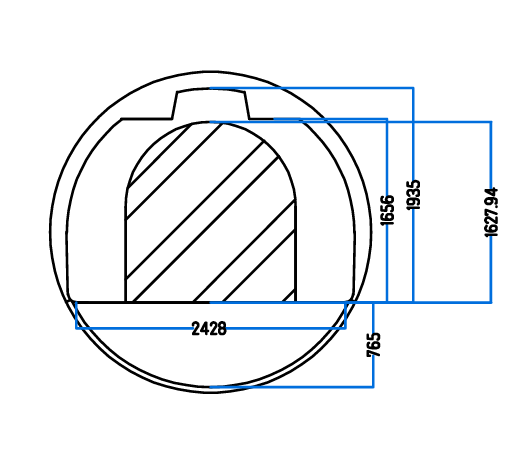
\includegraphics[width=0.4\linewidth]{images/palete_frontal.png}
    \caption{Vista Frontal}
    \label{fig:palete_frontal}
\end{figure}

\begin{figure}[H]
    \centering
    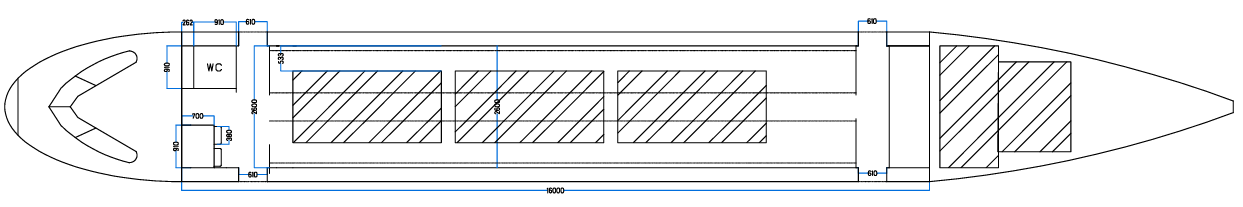
\includegraphics[width=1\linewidth]{images/palete_superior.png}
    \caption{Vista Superior}
    \label{fig:palete_superior}
\end{figure}

A transição rápida entre as configurações é viabilizada pela utilização dos trilhos estruturais mencionados na seção anterior. O piso da aeronave é equipado com trilhos universais de alta resistência, operando da seguinte forma:

\begin{itemize}
    \item \textbf{Configuração de Passageiros:} Os assentos são montados sobre "paletes de assento" (seat pallets) que se travam diretamente nos trilhos. Isso permite que as fileiras sejam removidas em blocos, minimizando o tempo de solo (\textit{turnaround}).
    \item \textbf{Configuração de Carga:} Após a remoção dos assentos, os mesmos trilhos recebem os \textit{locks} (travas) mecânicos para fixação dos paletes PLA. Para a movimentação interna, o piso integra esferas e roletes escamoteáveis (\textit{omni-directional rollers}), que permitem o deslize manual de cargas de até 3175 kg com esforço reduzido da equipe de solo.
\end{itemize}


\section{Geometria da Asa}

A fim de validar as escolhas de projeto abordadas teoricamente, realizou-se um levantamento estatístico restrito aos seis concorrentes diretos previamente selecionados (ATR 72-600, CASA C-295, Il-114-300, BAe ATP, NAMC YS-11 e Xian MA600). A Figura \ref{fig:pie_posicao_asa} ilustra a distribuição de mercado referente à posição da asa dessas aeronaves.

\begin{figure}[H]
    \centering
    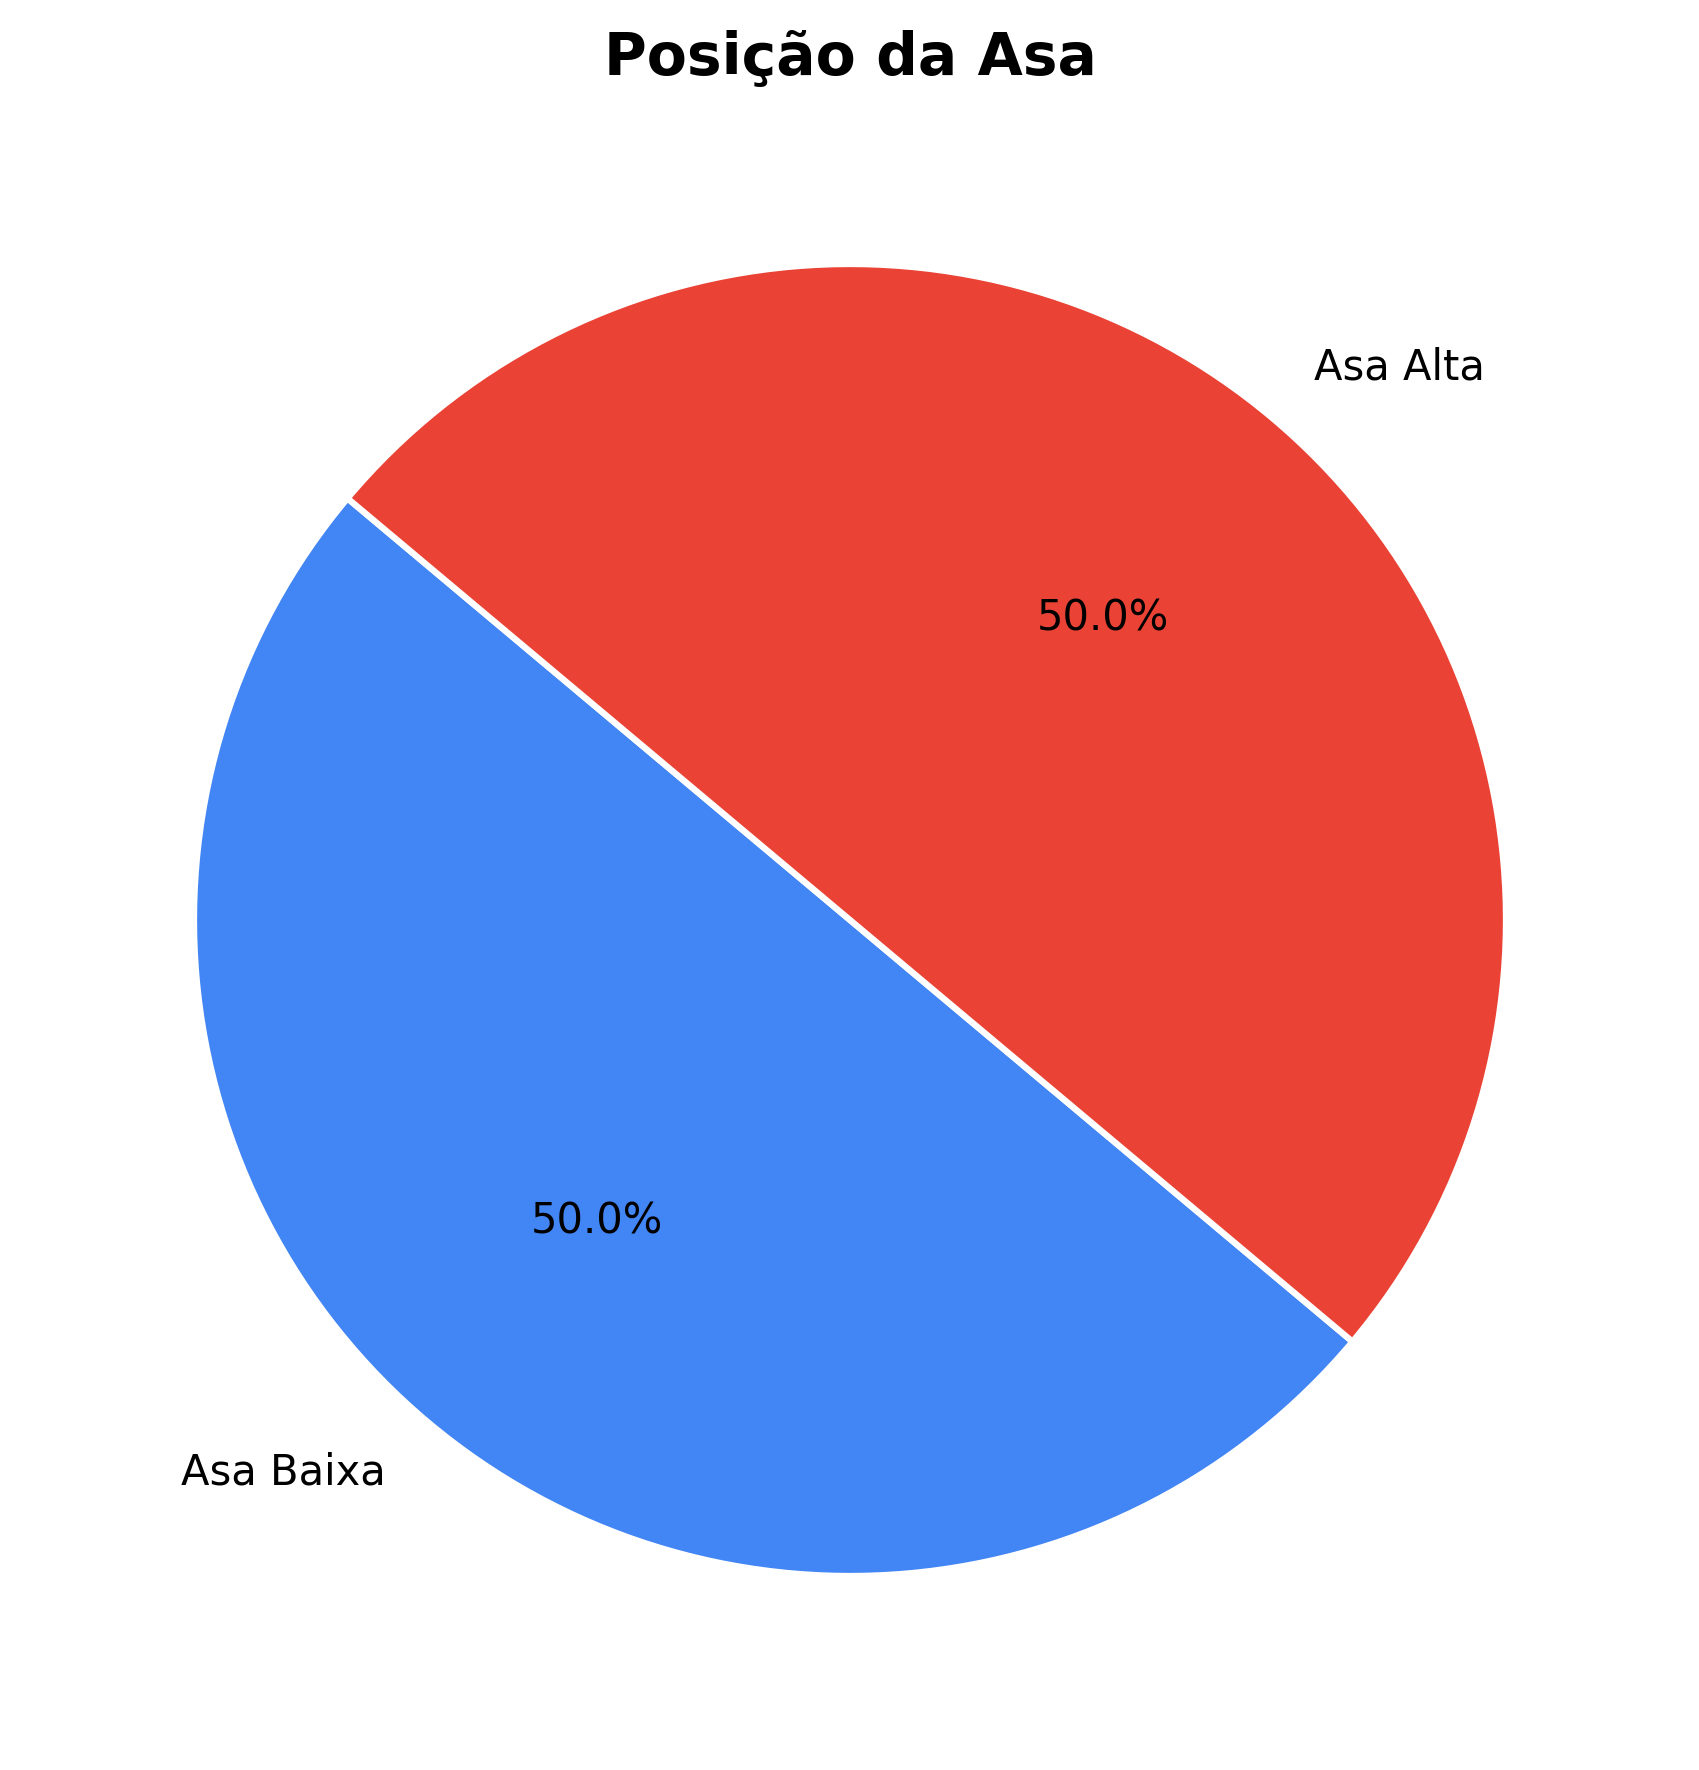
\includegraphics[width=0.4\linewidth]{Images-2-EstudoConceitual/pizza_asa.png} % Ajuste o caminho se necessário
    \caption{Distribuição da posição da asa entre os concorrentes diretos.}
    \label{fig:pie_posicao_asa}
\end{figure}

Conforme os dados apresentados, não há um consenso absoluto no mercado regional quanto à posição da asa, havendo um empate exato (50\% para cada) entre a adoção de asa alta e asa baixa. No entanto, corroborando a teoria de Anderson \cite{anderson1999}, a configuração de asa alta foi a selecionada para consolidar o Projeto Conceitual. Essa escolha alinha-se aos modelos de maior sucesso comercial e versatilidade (como o ATR 72 e o C-295), favorece o embarque de mercadorias em pistas com infraestrutura escassa e garante o distanciamento seguro das hélices de grande diâmetro em relação ao solo.

No que tange à geometria da planta, observa-se, dentre as aeronaves de referência, uma adoção única de formas trapezoidais entre o grupo de competidores avaliado. Essa unanimidade fundamenta-se no excelente compromisso aerodinâmico alcançado: a asa trapezoidal permite uma boa aproximação da distribuição de sustentação elíptica ideal (que minimiza drasticamente o arrasto induzido), ao mesmo tempo em que apresenta custos e complexidades de manufatura substancialmente menores quando comparada às asas elípticas ou compostas. Portanto, guiado pelas tendências das aeronaves de referência, este projeto adotará uma asa alta de geometria trapezoidal.

O ângulo de enflechamento definido foi zero, uma vez que seus principais benefícios estão associados a regimes transônicos e supersônicos, não sendo necessários para a faixa de velocidades prevista para a aeronave. Para o diedro, optou-se pela utilização de anedro, com \(\Gamma=-2,8^\circ\). Essa escolha está associada à configuração de asa alta adotada, que naturalmente apresenta um efeito estabilizante lateral pronunciado. A introdução de um anedro moderado permite reduzir esse efeito restaurador, proporcionando uma resposta mais adequada aos comandos de rolamento e evitando uma estabilidade lateral excessiva. O valor adotado constitui uma estimativa preliminar de projeto, devendo sua adequação ser posteriormente verificada nas análises de estabilidade látero-direcional da aeronave.

\begin{itemize}
    \item Raiz da Asa: NACA 43018
    \item Ponta da Asa: NACA 43013

\end{itemize}

Além disso, as dimensões das superfícies de comando da asa também foram baseadas nessa aeronave. Para envergadura, corda da raiz e corda da ponta, foi calculada a média entre os valores extremos para essas dimensões nas seis aeronaves semelhantes. Esse método permite utilizar de forma mais direta a amplitude do envelope de projeto praticado pelos concorrentes, garantindo que a aeronave seja competitiva dentro dos limites operacionais já validados pelo mercado. Os valores desses parâmetros são apresentados na tabela \ref{tab:dimensões da asa}.

\begin{table}[H]
  \centering
  \linespread{1}\small
  \setlength{\tabcolsep}{4pt}
  \caption{Parâmetros geométricos da asa e superfícies de controle.}
  \label{tab:dimensões da asa}
  \begin{tabularx}{\textwidth}{L C}
    \toprule
    \textbf{Dimensão} & \textbf{Valor} \\
    \midrule
    Envergadura (b) & 28,5 m \\
    Corda da raiz & 3,7 m \\
    Corda da ponta & 1,5 m \\
    Aileron & 3,8 m (comp.) / 0,92 m (larg.) \\
    Flap & 8,7 m (comp.) / 0,44 m (larg.) \\
    \bottomrule
  \end{tabularx}
\end{table}

Por fim, o afilamento, o alongamento, a área alar e a corda média aerodinâmica foram calculados pelas relações geométricas clássicas dadas pelas equações \eqref{área alar} a \eqref{corda média aerodinâmica}, usando os valores determinados no processo descrito anteriormente.

\begin{equation}
S = \frac{b \, (c_{raiz} + c_{ponta})}{2} = \frac{28,5 \cdot (3,7 + 1,5)}{2} = 74,1 \, m^2
\label{área alar}
\end{equation}

\begin{equation}
\lambda = \frac{c_{ponta}}{c_{raiz}} = \frac{1,5}{3,7} \approx 0,405
\label{afilamento}
\end{equation}

\begin{equation}
AR = \frac{b^2}{S} = \frac{28,5^2}{74,1} \approx 10,96
\label{alongamento}
\end{equation}

\begin{equation}
\bar{c} = \frac{2}{3} \, c_{raiz} \, \frac{1 + \lambda + \lambda^2}{1 + \lambda} = \frac{2}{3} \cdot 3,7 \cdot \frac{1 + 0,405 + 0,405^2}{1 + 0,405} \approx 2,75 \, m
\label{corda média aerodinâmica}
\end{equation}

%%%%%%%%%%%%%%%%%%%%%%%%%%%%%%%%%%%%%%%%%%%%%%%%%%%%%%%%%%%%%%%%%%%%%
%%%%%%%%%%%%%%%%%%%%%%%%%%%%%%%%%%%%%%%%%%%%%%%%%%%%%%%%%%%%%%%%%%%%%
%%%%%%%%%%%%%%%%%%%%%%%%%%%%%%%%%%%%%%%%%%%%%%%%%%%%%%%%%%%%%%%%%%%%%

\section{Geometria da Empenagem}
Para embasar a seleção da arquitetura de cauda, avalia-se a tendência adotada pelas aeronaves de referência concorrentes. A Figura \ref{fig:tipo_empenage} mostra que 83,3\% adotam empenagem convencional, sendo o ATR 72-600 a única exceção entre os concorrentes diretos.

\begin{figure}[htbp]
    \centering
    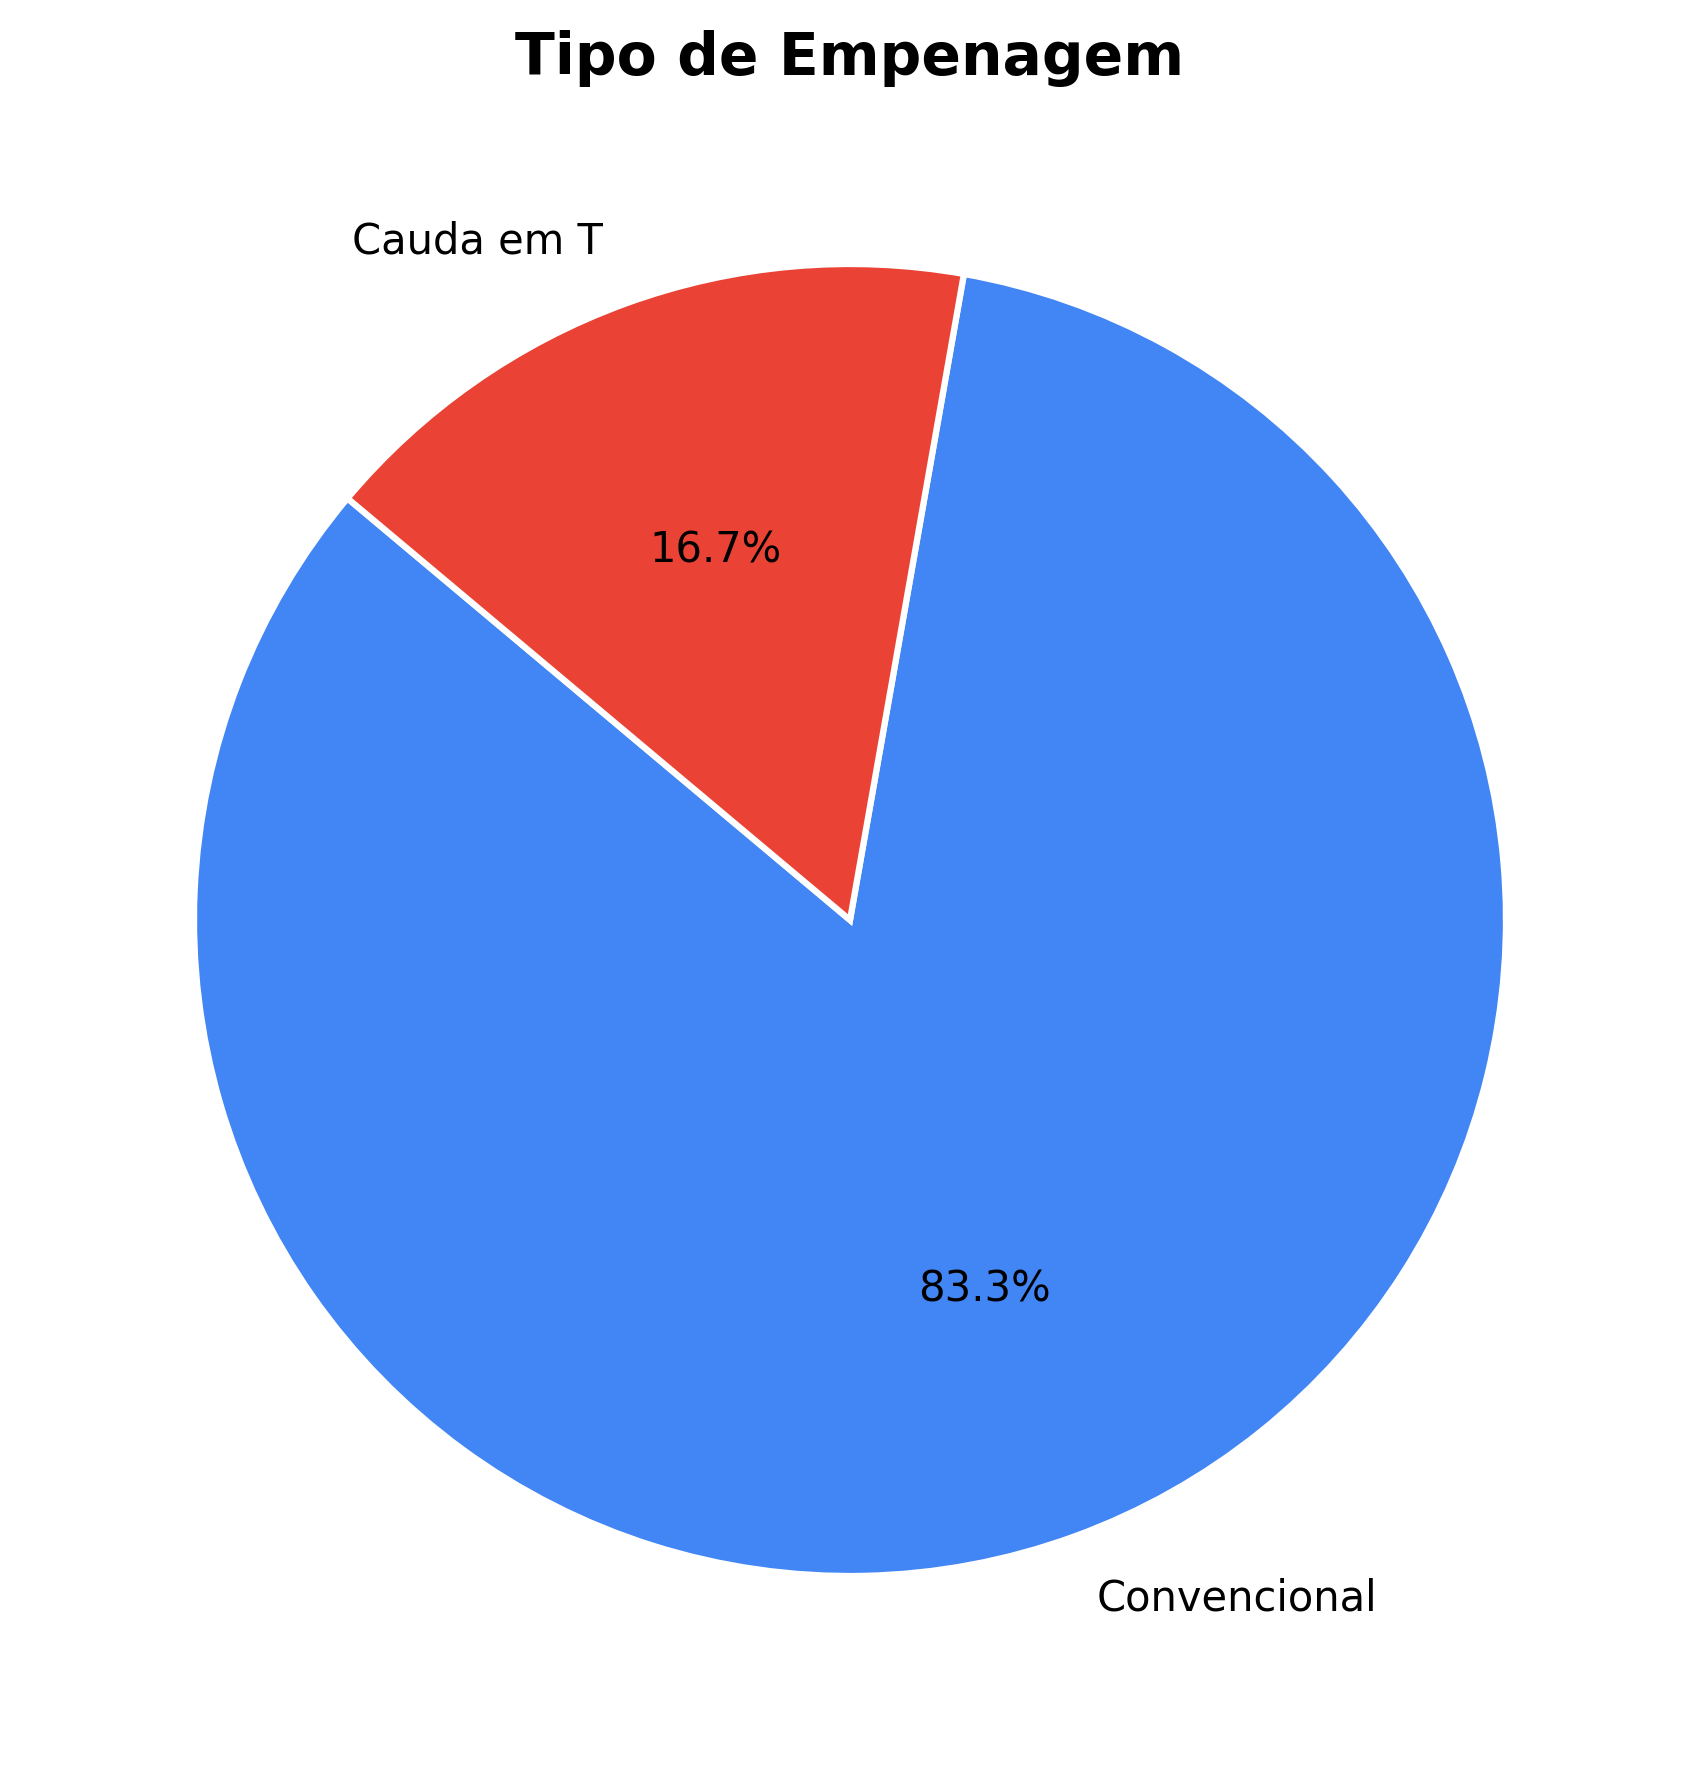
\includegraphics[width=0.6\textwidth]{Images-2-EstudoConceitual/pizza_empenagem.png} 
    \caption{Distribuição do tipo de empenagem entre os concorrentes diretos.}
    \label{fig:tipo_empenage}
\end{figure}

A cauda em T posiciona a empenagem horizontal no topo da empenagem vertical, afastado da esteira da asa e do escoamento das hélices. Em alto ângulo de ataque, porém, a esteira de baixa energia da asa e da fuselagem pode envolver a empenagem horizontal, reduzindo drasticamente a autoridade do profundor e podendo conduzir ao \textit{deep stall}, condição na qual a recuperação por comandos convencionais pode ser comprometida \cite{nguyen2023}. Essa susceptibilidade é agravada pela configuração de asa alta. Para mitigá-la, a cauda em T pode requerer sistemas de prevenção de estol, como o \textit{stick pusher} utilizado no ATR 72-600, com acréscimo de peso, custo de certificação e verificações periódicas.


\begin{figure}[H]
    \centering
    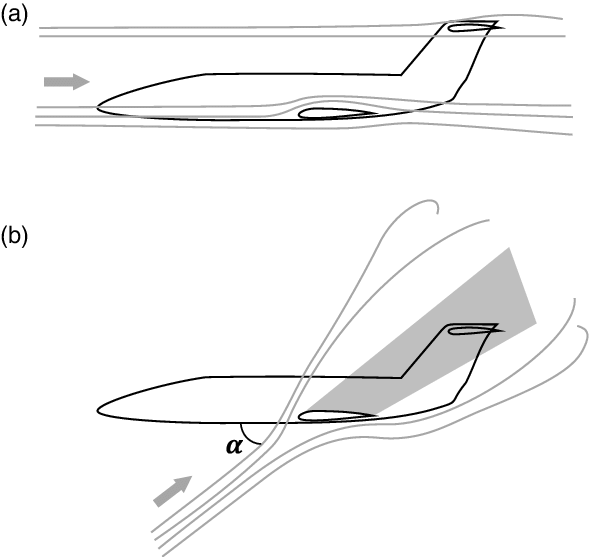
\includegraphics[width=0.7\textwidth]{Images-2-EstudoConceitual/deep_stall_wake.png} 
    \caption{Aeronave de cauda em T (a) em voo normal e (b) em condição de \textit{deep stall}, com a região de esteira de baixa energia da asa (área sombreada) envolvendo a empenagem horizontal em alto ângulo de ataque $\alpha$. Adaptado de \cite{nguyen2023}.}
    \label{fig:deep_stall}
\end{figure}

Na configuração convencional, a empenagem horizontal é fixada ao cone de cauda e permanece abaixo da esteira da asa em alto ângulo de ataque. Isso preserva a autoridade do profundor e favorece a recuperação natural do estol, dispensando sistema dedicado de prevenção. Os carregamentos das empenagens horizontal e vertical ficam desacoplados, o que simplifica o dimensionamento estrutural. Além disso, parte da empenagem horizontal opera no escoamento acelerado pelas hélices, o que aumenta a eficácia do profundor em baixa velocidade e alta potência, condição da decolagem, fase crítica do projeto (distância calculada de 1.102~m contra requisito de 1.280~m). Como contrapartida, a empenagem fica na região de \textit{downwash} da asa, o que exige área ligeiramente maior. Esse efeito é aceito diante dos ganhos descritos. O CASA C-295, de MTOW de 23.200~kgf e com grupo motopropulsor da mesma família deste projeto, adota empenagem convencional.

Dessa forma, a configuração convencional é a escolhida, por dispensar sistema dedicado de prevenção de estol, por favorecer a recuperação inerente do estol e por estar alinhada à tendência das aeronaves de referência. O perfil adotado para a empenagem horizontal é o NACA 0012, simétrico, por não gerar sustentação a ângulo de ataque nulo e por dispor de ampla base de dados experimentais. Para a empenagem vertical, adota-se o NACA 0010, de espessura relativa menor que a do horizontal.





%%%%%%%%%%%%%%%%%%%%%%%%%%%%%%%%%%%%%%%%%%%%%%%%%%%%%%%%%%%%%%%%%%%%%
%%%%%%%%%%%%%%%%%%%%%%%%%%%%%%%%%%%%%%%%%%%%%%%%%%%%%%%%%%%%%%%%%%%%%
%%%%%%%%%%%%%%%%%%%%%%%%%%%%%%%%%%%%%%%%%%%%%%%%%%%%%%%%%%%%%%%%%%%%%

\section{Escolha da Propulsão}

A fim de dimensionar preliminarmente a motorização da aeronave e correlacioná-la com os requisitos de projeto estipulados e com os dados das aeronaves de referência, foram geradas as Figuras \ref{fig:pot_mtow} e \ref{fig:dec_pot}. Neste trabalho, as potências dos motores turboélice são expressas em \textit{shaft horsepower} (SHP), isto é, potência mecânica disponível no eixo do motor.

A Figura \ref{fig:pot_mtow} ilustra a tendência de potência total instalada em função do MTOW na classe de aeronaves estudada. O requisito estabelecido para este projeto prevê um MTOW de 22.680 kgf (indicado pela linha tracejada vermelha). Observando a dispersão estatística e a linha de tendência linear do mercado, conclui-se que o projeto exigirá uma potência total no eixo na faixa de 5.000 a 5.300 shp (aproximadamente 2.500 a 2.650 shp por motor). Este patamar é fundamental para manter a carga de potência ($W/P$) em um nível competitivo e garantir o desempenho em subida.

\begin{figure}[H]
    \centering
    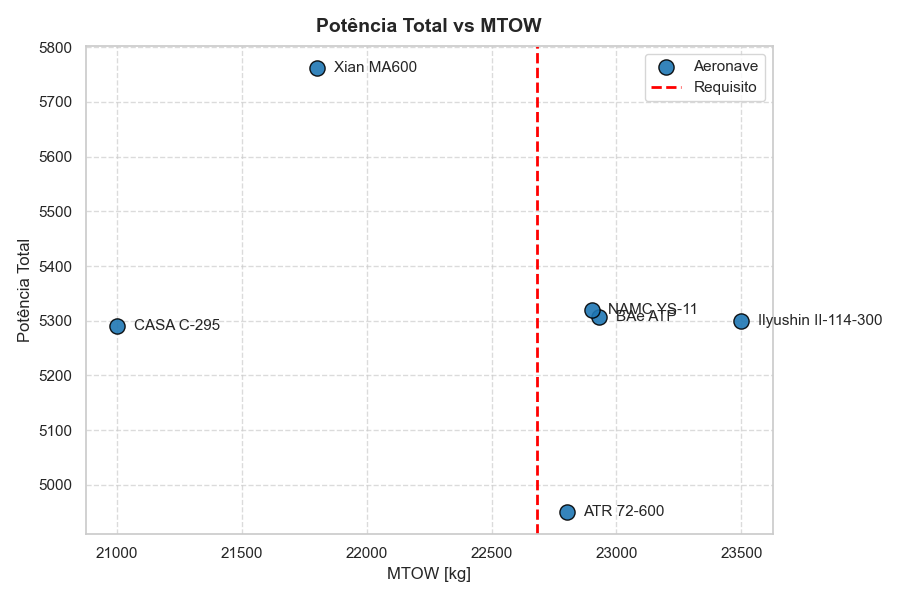
\includegraphics[width=0.75\linewidth]{Images-2-EstudoConceitual/pot_x_mtow.png}
    \caption{Correlação entre Potência Total Instalada e MTOW nos concorrentes diretos.}
    \label{fig:pot_mtow}
\end{figure}

A justificativa para garantir esse nível de potência é diretamente validada pelo rigoroso requisito de decolagem do projeto, estipulado em um comprimento máximo de 1.280 m. A Figura \ref{fig:dec_pot} correlaciona o desempenho de pista das aeronaves de referência com suas respectivas motorizações, evidenciando o limite imposto pelo requisito (linha vermelha tracejada). 

\begin{figure}[H]
    \centering
    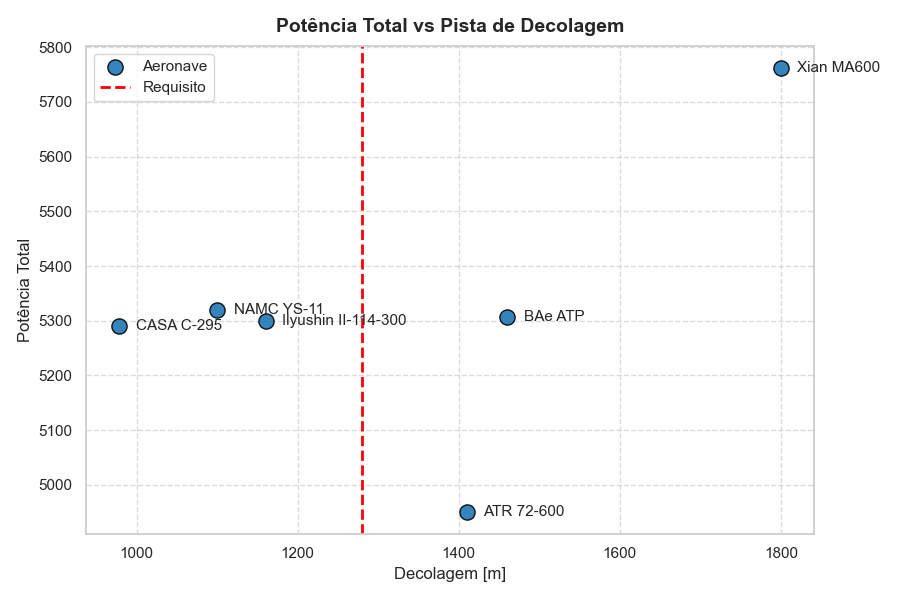
\includegraphics[width=0.75\linewidth]{Images-2-EstudoConceitual/pot_x_decolagem.png}
    \caption{Desempenho de decolagem das aeronaves de referência em função da potência instalada.}
    \label{fig:dec_pot}
\end{figure}

Para garantir que o protótipo opere com folga dentro dos 1.280 m sob condições críticas, a potência estimada na Figura \ref{fig:pot_mtow} precisará atuar em conjunto com um sistema hipersustentador (flaps) de alta eficiência e um conjunto de hélices otimizado para tração estática.

Por fim, o motor selecionado para o projeto da aeronave foi o PW127M, por atender plenamente as necessidades da missão proposta, além de ser da família de motores mais presente nas análises comparativas, o que reforça a confiabilidade e adequação ao projeto. Para além das análises comparativas, o motor da \textit{Pratt \& Whitney} dispõe de relatórios e manuais disponíveis na internet, com informação suficiente para as análises e dimensionamentos posteriores.

Conforme os dados oficiais de certificação estabelecidos no Type Certificate Data Sheet (TCDS) da família PW100 (FAA TCDS nº E20NE / EASA TCDS nº E.070) e no Manual do Fabricante (Part No. 3037332), o motor PW127M é homologado para fornecer uma potência termodinâmica máxima de decolagem de 2.475 shp por unidade. Essa capacidade resulta em uma potência total instalada de 4.950 shp, atendendo plenamente à demanda requerida (entre 5.000 e 5.300 shp, com as devidas margens) para a operação da aeronave nas curtas distâncias de pista estabelecidas pelos requisitos do projeto.

A Tabela~\ref{tab:pw127m} consolida os parâmetros técnicos principais do motor PW127M, confrontando-os com os requisitos de projeto. Nota-se que a potência total instalada de 4.950 shp posiciona a aeronave dentro da faixa prevista pela análise estatística da Figura~\ref{fig:pot_mtow}, e a carga de potência resultante ($W/P \approx 4{,}58$ kg/shp) é competitiva com os concorrentes diretos, em especial o ATR~72-600, cujo motor é o mesmo modelo. 

A combinação do PW127M com as hélices Hamilton Standard 568F, já validadas operacionalmente no ATR~72-600, e com o sistema de flaps dimensionado na seção anterior constitui a solução propulsiva capaz de cumprir o requisito de MTOW e de decolagem.

\begin{table}[H]
  \centering
  \linespread{1}\small
  \setlength{\tabcolsep}{4pt}
  \caption{Parâmetros técnicos do motor selecionado (PW127M) e sua conformidade com os requisitos de projeto.}
  \label{tab:pw127m}
  \begin{tabularx}{\textwidth}{>{\hsize=1.2\hsize}L >{\hsize=0.9\hsize}C >{\hsize=0.9\hsize}C}
    \toprule
    \textbf{Parâmetro} & \textbf{Valor} & \textbf{Requisito / Referência} \\
    \midrule
    Fabricante & Pratt \& Whitney Canada & --- \\
    Modelo & PW127M & --- \\
    Tipo & Turboélice & Turboélice (seção 3.2.4) \\
    Número de motores & 2 & 2 (seção 3.2.4) \\
    Potência máx.\ de decolagem (por motor) & 2.475 shp & $\geq$ 2.500 shp (est.) \\
    Potência total instalada & 4.950 shp & 5.000--5.300 shp (Fig.~\ref{fig:pot_mtow}) \\
    Peso seco por motor & 480,8 kgf (1.060 lb) & --- \\
    Carga de potência ($W/P$) & 4,58 kg/shp & Compatível com concorrentes \\
    Hélice & Hamilton Standard 568F & --- \\
    Pista de decolagem estimada & $\leq$ 1.280 m & $\leq$ 1.280 m (seção 2.1) \\
    Velocidade de cruzeiro compatível & 260 kt & 260 kt (seção 2.1) \\
    Teto de serviço compatível & FL250 & FL250 (seção 2.1) \\
    \bottomrule
  \end{tabularx}
\end{table}

Definido o conjunto motopropulsor deste projeto (motor PW127M acoplado à hélice Hamilton Standard 568F de 6 pás), cabe justificar tecnicamente essa escolha frente à alternativa de 4 pás, historicamente empregada em variantes de menor potência da mesma família de referência. De forma que essa decisão impacta diretamente a eficiência propulsiva, nível de ruído e vibração de cabine, peso do grupo  motopropulsor e a integridade estrutural da pá frente a efeitos de compressibilidade. A Tabela \ref{tab:comparativo_pas} sintetiza a comparação técnica entre as duas configurações consideradas.

\begin{table}[H]
  \centering
  \linespread{1}\small
  \setlength{\tabcolsep}{4pt}
  \caption{Comparativo entre hélices de 4 e 6 pás para a faixa de potência do projeto.}
  \label{tab:comparativo_pas}
  \begin{tabularx}{\textwidth}{L L L}
    \toprule
    \textbf{Critério} & \textbf{4 pás} & \textbf{6 pás} \\
    \midrule
    Peso do conjunto rotativo & Menor & Maior \\
    Complexidade/custo de manutenção & Menor & Maior \\
    Absorção de potência (diâmetro fixo) & Limitada & Adequada \\
    Velocidade de ponta / compressibilidade & Prejudicial em alta potência & Mitigada \\
    Ruído e vibração de cabine & Maior & Menor (37, 38) \\
    Precedente na potência do projeto & ATR 72-200, PW124B ($\sim$2.400 shp) & ATR 72-500/600, PW127 ($\sim$2.475--2.750 shp) \\
    \bottomrule
  \end{tabularx}
\end{table}

Assim, a configuração de 4 pás apresenta vantagens de peso, custo e complexidade mecânica, que, no entanto, são características de motores na faixa de 2.000--2.400 shp por unidade, como o PW124B utilizado no ATR 72-200 com hélices Hamilton Standard 14SF-11. Para a potência efetivamente instalada neste projeto (motor PW127M), certificado sob a TCDS E20NE da FAA para a família PW100, com 2.475 shp por motor (Tabela \ref{tab:pw127m}), os critérios que passam a dominar a decisão são aqueles em que a configuração de 6 pás se sobressai: capacidade de absorção de potência sem penalizar a velocidade de ponta e o ruído de cabine. Esse comportamento é consistente com a evolução real da família ATR, que substituiu a hélice de 4 pás pela Hamilton Standard 568F de 6 pás ao migrar do PW124B para o PW127M, mantendo o diâmetro praticamente inalterado conforme a TCDS P8BO da Hamilton Sundstrand Corp. e o comunicado técnico da Collins Aerospace, atual fabricante do conjunto, que reporta mais de 30 milhões de horas de voo em serviço nessa configuração de 6 pás na frota ATR 42/72.

Para uma dada rotação, uma hélice absorve mais potência apenas por dois caminhos: aumentar o diâmetro (elevando diretamente a componente rotacional da velocidade de ponta, $V_{rot} = \pi \cdot D \cdot N$) ou aumentar a solidez do disco, absorvendo mais potência sem penalizar essa velocidade. Utilizando os dados de diâmetro e rotação de referência da hélice 568F ($D = 3{,}93$ m; $N \approx 1200$ rpm a 100\% $N_p$, conforme especificação do fabricante do motor (36)) na condição de cruzeiro do projeto ($V_{cruise} = 260$ kt; FL250 -- Tabela \ref{tab:pw127m}), obtém-se:

\begin{equation}
    V_{rot} = \pi \cdot D \cdot N = \pi \cdot 3{,}93 \cdot \left(\frac{1200}{60}\right) 
\approx 247 \text{ m/s}
    \label{eq:vrot}
\end{equation}

\begin{equation}
    V_{ponta} = \sqrt{V_{rot}^2 + V_{cruise}^2} = \sqrt{247^2 + 133{,}8^2} 
    \approx 281 \text{ m/s}
    \label{eq:vponta}
\end{equation}

Para a atmosfera padrão ISA em FL250 ($T \approx 238{,}7$ K), a velocidade do som é $a \approx 310$ m/s, resultando em um número de Mach de ponta de pá de:

\begin{equation}
    M_{ponta} = \frac{V_{ponta}}{a} \approx 0{,}91
    \label{eq:mach_ponta}
\end{equation}

Esse valor já se encontra próximo do limite prático de operação subsônica na ponta da pá, mesmo com 6 pás absorvendo a potência do PW127M. Caso a mesma potência fosse absorvida por apenas 4 pás no mesmo diâmetro, seria necessário aumentar a corda/espessura de cada pá para preservar a área projetada total, elevando a aceleração local do escoamento, aumentando ainda mais esse número de Mach efetivo. Alternativamente, aumentar o diâmetro eleva diretamente $V_{rot}$ na Equação \ref{eq:vrot} e, consequentemente, $V_{ponta}$ na Equação \ref{eq:vponta}. Esse comportamento apresenta perdas por compressibilidade e aumento de ruído tonal proporcionais ao número de Mach helicoidal de ponta como apresentado na literatura técnica sobre hélices de alta velocidade.

Diante do exposto na Tabela \ref{tab:comparativo_pas} e da verificação quantitativa acima, mantém-se a adoção da hélice Hamilton Standard 568F de 6 pás para este projeto. Embora a configuração de 4 pás seja tecnicamente superior em peso e custo, ela é adequada apenas à faixa de potência de motores como o PW124B, inferior à do PW127M a ser adotado. Para a potência e o diâmetro que caracterizam esta aeronave, a configuração de 6 pás é a que melhor concilia absorção de potência, integridade estrutural da pá e conforto de cabine, replicando a mesma solução já validada operacionalmente pela família ATR 72-500/600 nessa exata faixa de potência.

\subsection{Integração da Hélice e Distância ao Solo}
\label{sec:selecao_pas}

Para garantir a segurança operacional e o cumprimento dos requisitos de certificação, procedeu-se à verificação da distância vertical entre a ponta da pá da hélice e o solo (ground clearance). O \S 25.925(a) do 14 CFR Part 25 determina que, para aeronaves com trem de pouso triciclo, a distância mínima entre a hélice e o solo deve ser de pelo menos 7 polegadas (178 mm) com a aeronave estática no peso máximo.  

Na configuração adotada para esta aeronave de asa alta, a linha de centro dos motores (eixo da hélice) encontra-se alinhada ao topo da fuselagem. Sabendo que o diâmetro da fuselagem é de 2.900 mm e a altura estática do trem de pouso dimensionado é de 700 mm, a altura total do eixo do motor em relação ao solo é de 3.600 mm.  A hélice selecionada, Hamilton Standard 568F, possui um diâmetro de 3,93 m, o que resulta em um raio de 1.965 mm. A distância vertical da ponta da pá ao solo é calculada subtraindo-se o raio da hélice da altura do eixo do motor: 

$Clearance = H_{motor} - R_{prop}$

$Clearance = 3.600 \text{ mm} - 1.965 \text{ mm} = 1.635 \text{ mm} \text{ (ou } 1,635 \text{ m)}$

O valor obtido de 1.635 mm supera o mínimo normativo de 178 mm. Essa folga vertical é uma vantagem do projeto, pois mitigará o risco de ingestão ou impacto de detritos, uma característica fundamental para uma aeronave regional projetada para operar em aeroportos com infraestrutura limitada ou pistas semi-preparadas.

\subsection{Segurança, Marcação e Posicionamento do Disco da Hélice}
\label{sec:seguranca_helice}

No que tange à segurança e certificação, o posicionamento das hélices Hamilton Standard 568F foi avaliado frente a cenários de falha catastrófica (como a perda de uma pá) e ao desprendimento de gelo (ice shedding). Conforme o \S 25.903(d) do 14 CFR Part 25, o projeto deve minimizar os riscos aos ocupantes em caso de falha de rotores.

Analisando o arranjo geral da aeronave, o plano de rotação do disco da hélice cruza a fuselagem na zona de serviço dianteira, região que abriga o lavatório e os compartimentos de bagagem. Essa disposição geométrica é altamente vantajosa, pois o plano do disco não intercepta diretamente a cabine de comando (cockpit) nem as fileiras de assentos dos passageiros. Para mitigar o impacto de blocos de gelo desprendidos das pás pela força centrífuga, a seção da fuselagem alinhada ao disco da hélice deverá ser estruturalmente reforçada com a instalação de painéis externos de impacto (ice shields).

Adicionalmente, para garantir a segurança das equipes de apoio e handling durante as operações em solo com os motores em funcionamento, são adotadas medidas de sinalização visual padronizadas. As pontas das pás das hélices receberão pintura de segurança em cores de alto contraste (faixas concêntricas de amarelo, preto e branco ou vermelho e branco), criando um arco visual contínuo e facilmente identificável quando em rotação. Em complemento, a superfície externa da fuselagem receberá marcações de aviso com faixas verticais vermelhas ladeando o plano do disco, acompanhadas da inscrição "PROPELLER" e setas de advertência, em conformidade com as exigências de segurança de rampa.

\chapter{Estudo de Conversão}

\section{Análise de Aeronaves de Referência}

O desenvolvimento do conceito de operação em missão dupla exige uma arquitetura de cabine que minimize o tempo de pátio durante o processo de reconfiguração. Na análise de projetos consolidados, observam-se filosofias distintas para a solução deste problema.

Aeronaves regionais civis tradicionais, como o ATR-72, quando adaptadas para operações de carga ou conversões rápidas, dependem da extração de assentos e inserção de cargas através de portas laterais. Na versão \textit{Quick Change} ou nos layouts convertíveis do ATR-72, o processo logístico exige a movimentação de componentes unitários através de aberturas dispostas lateralmente na fuselagem. O processo oficial de conversão de cabine leva em torno de uma hora no ATR-72, sendo frequentemente planejado como um procedimento para as janelas noturnas.

Em geral, no procedimento de conversão, a equipe de solo inicia com a desmontagem manual de elementos de cabine, como os painéis de divisão, as redes de contenção e o assento dianteiro do comissário. Após o destravamento mecânico das fileiras de assentos, que são instaladas de modo convencional nos trilhos do piso, estas fileiras são transladadas manualmente ao longo do corredor central em direção às saídas operacionais. A remoção das poltronas para o exterior e a inserção da carga paletizada ocorre através de uma porta de carga alargada (conhecida como \textit{Large Cargo Door}). Esta porta dispõe de uma soleira rebaixada a uma certa altura do solo para facilitar o recebimento dos contêineres otimizados.  

Embora o sistema QC atenda às normas e permita ao ATR acomodar ULDs no main deck, a cinemática de conversão por portas laterais exigem que os assentos e paletes extraídos precisem ser rotacionados em 90 graus no interior da aeronave antes de passarem pelo vão da porta, o que demanda maior intervenção braçal e expõe o revestimento interno a danos.

Tomando como outro exemplo a aeronave CASA C-295, originada como um cargueiro tático, apresenta uma arquitetura intrinsecamente modular, resolvendo o gargalo direcional através de uma rampa traseira e um piso plano provido de um sistema contínuo de roletes e pontos de fixação compatíveis com paletes. A transição total da cabine de carga para uma configuração completa e segura de passageiros ou transporte aeromédico pode ser finalizada em menos de 2 horas.

Em geral, os assentos de passageiros são fixados previamente de forma integral sobre plataformas padronizadas de assoalho (como o sistema multibase), juntamente com equipamentos auxiliares de oxigênio e segurança. A montagem estrutural de cada palete fora da aeronave é rápida, exigindo apenas dois operadores e cerca de 20 minutos. Para a inserção, a rampa traseira principal atua como a interface direta entre o nível de carregamento e a cabine, podendo operar nivelada com equipamentos de rampa de solo. O translado logístico dos grandes paletes modulares é realizado com o auxílio de um guincho mecânico no interior da cabine. Finalmente, os paletes contendo os assentos são fixados de modo consolidado no piso, sem a necessidade de acoplar as fileiras individualmente.

Essa solução longitudinal ininterrupta suprime a extração avulsa e contorna as limitações de rotação das portas laterais. Contudo, é importante ponderar as penalidades de projeto inerentes a esta arquitetura. A necessidade de uma rampa traseira pressurizável e de um assoalho com trilhos estruturais eleva substancialmente o peso vazio operacional (OEW) da aeronave, além de o formato elevado da cauda impor um incremento considerável de arrasto aerodinâmico de base.

\section*{Escolha e Justificativa da Arquitetura de Carregamento}

Para este projeto, optou-se pela implementação de uma porta de carga lateral (\textit{Large Cargo Door} - LCD) em detrimento de uma rampa de carregamento traseira. Do ponto de vista da integração estrutural, a porta lateral é significativamente mais simples de projetar e manufaturar, pois preserva a geometria cilíndrica convencional da fuselagem. A adoção de uma porta traseira exigiria o projeto de um cone de cauda elevado, o que não apenas incrementa o arrasto aerodinâmico de base, mas também pode alterar de forma indesejada as derivadas de estabilidade e a controlabilidade direcional e longitudinal da aeronave, exigindo um redimensionamento complexo da empenagem.

Adicionalmente, a filosofia de carregamento deve estar estritamente alinhada com o perfil da dupla missão proposta. Rampas traseiras, embora otimizem o tempo de transição, são mandatórias primordialmente para cargas indivisíveis de grande porte ou veículos táticos. Para uma aeronave comercial de transporte regional, cujas cargas consistem essencialmente em paletes padronizados e contêineres ULDs, a porta lateral se mostra a solução mais coerente. Essa escolha simplifica consideravelmente o planejamento aeroportuário, garantindo compatibilidade imediata com a infraestrutura civil existente e permitindo o uso de elevadores de carga e Equipamentos de Apoio no Solo (GSE) convencionais, amplamente disponíveis em aeroportos regionais.

Apesar da adoção da porta lateral, a filosofia de \textit{Quick Change} baseada no deslizamento longitudinal será mantida para maximizar a modularidade da cabine. As fileiras de assentos permanecerão fixadas aos trilhos estruturais do piso. Durante a conversão, os módulos de assentos serão destravados e transladados ao longo do corredor até a seção da porta. Para efetivar a transição física dos assentos e cargas entre o \textit{main deck} e o pátio, a operação dependerá da interface com plataformas elevatórias externas ou rampas móveis posicionadas ao lado da aeronave, compensando a ausência de uma rampa integrada sem penalizar o peso vazio operacional (OEW).

Por fim, é imperativo destacar as mitigações operacionais necessárias inerentes a esta arquitetura. A cinemática de carregamento por porta lateral exige uma inevitável mudança de direção: uma rotação de 90 graus dos paletes e módulos de assentos no interior da aeronave antes da extração. Consequentemente, a área do piso adjacente à porta deverá ser equipada com painéis de transferência omnidirecional e a equipe de \textit{handling} deverá adotar procedimentos rigorosos para evitar impactos e danos estruturais ao revestimento interno durante as manobras logísticas.

\section{Esboços Iniciais}

A seguir, são apresentadas as vistas principais da aeronave. Ressalta-se que essas representações correspondem a um esboço inicial do projeto, tendo como objetivo fornecer uma visualização preliminar da geometria.

% --- VISTA SUPERIOR ---
\begin{figure}[H]
    \centering
    \begin{minipage}{0.8\textwidth} % Ajuste o 0.8 para aumentar ou diminuir o tamanho
        \centering
        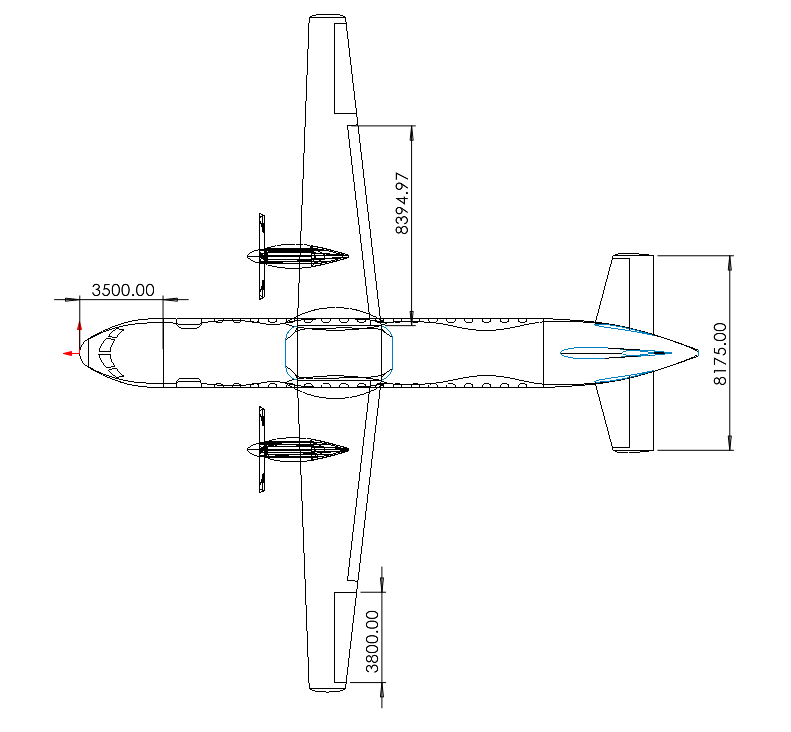
\includegraphics[width=\linewidth]{Images-2-EstudoConceitual/vista_superior.png}
        \caption{Esboço da vista superior da aeronave.}
        \label{fig:vista_superior}
    \end{minipage}
\end{figure}

% --- VISTA LATERAL ---
\begin{figure}[H]
    \centering
    \begin{minipage}{0.8\textwidth}
        \centering
        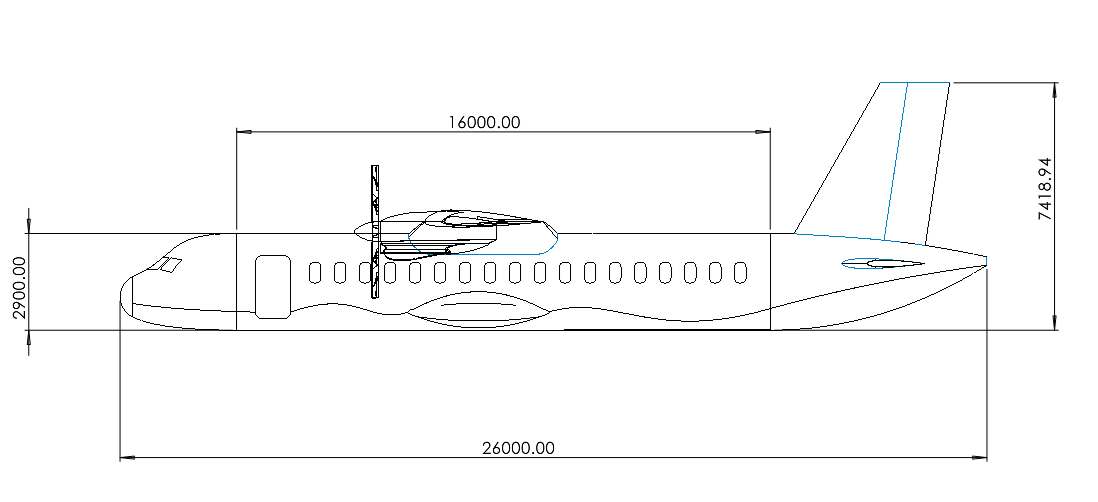
\includegraphics[width=\linewidth]{Images-2-EstudoConceitual/vista_lateral.png}
        \caption{Esboço da vista lateral da aeronave.}
        \label{fig:vista_lateral}
    \end{minipage}
\end{figure}

% --- VISTA FRONTAL ---
\begin{figure}[H]
    \centering
    \begin{minipage}{0.8\textwidth}
        \centering
        \includegraphics[width=\linewidth]{Images-2-EstudoConceitual/vista_frontal.png}
        \caption{Esboço da vista frontal da aeronave.}
        \label{fig:vista_frontal}
    \end{minipage}
\end{figure}

% --- VISTA ISOMÉTRICA (SEPARADA/DESTAQUE) ---
\begin{figure}[H]
    \centering
    \begin{minipage}{0.9\textwidth} % Isométrica levemente maior para destaque
        \centering
        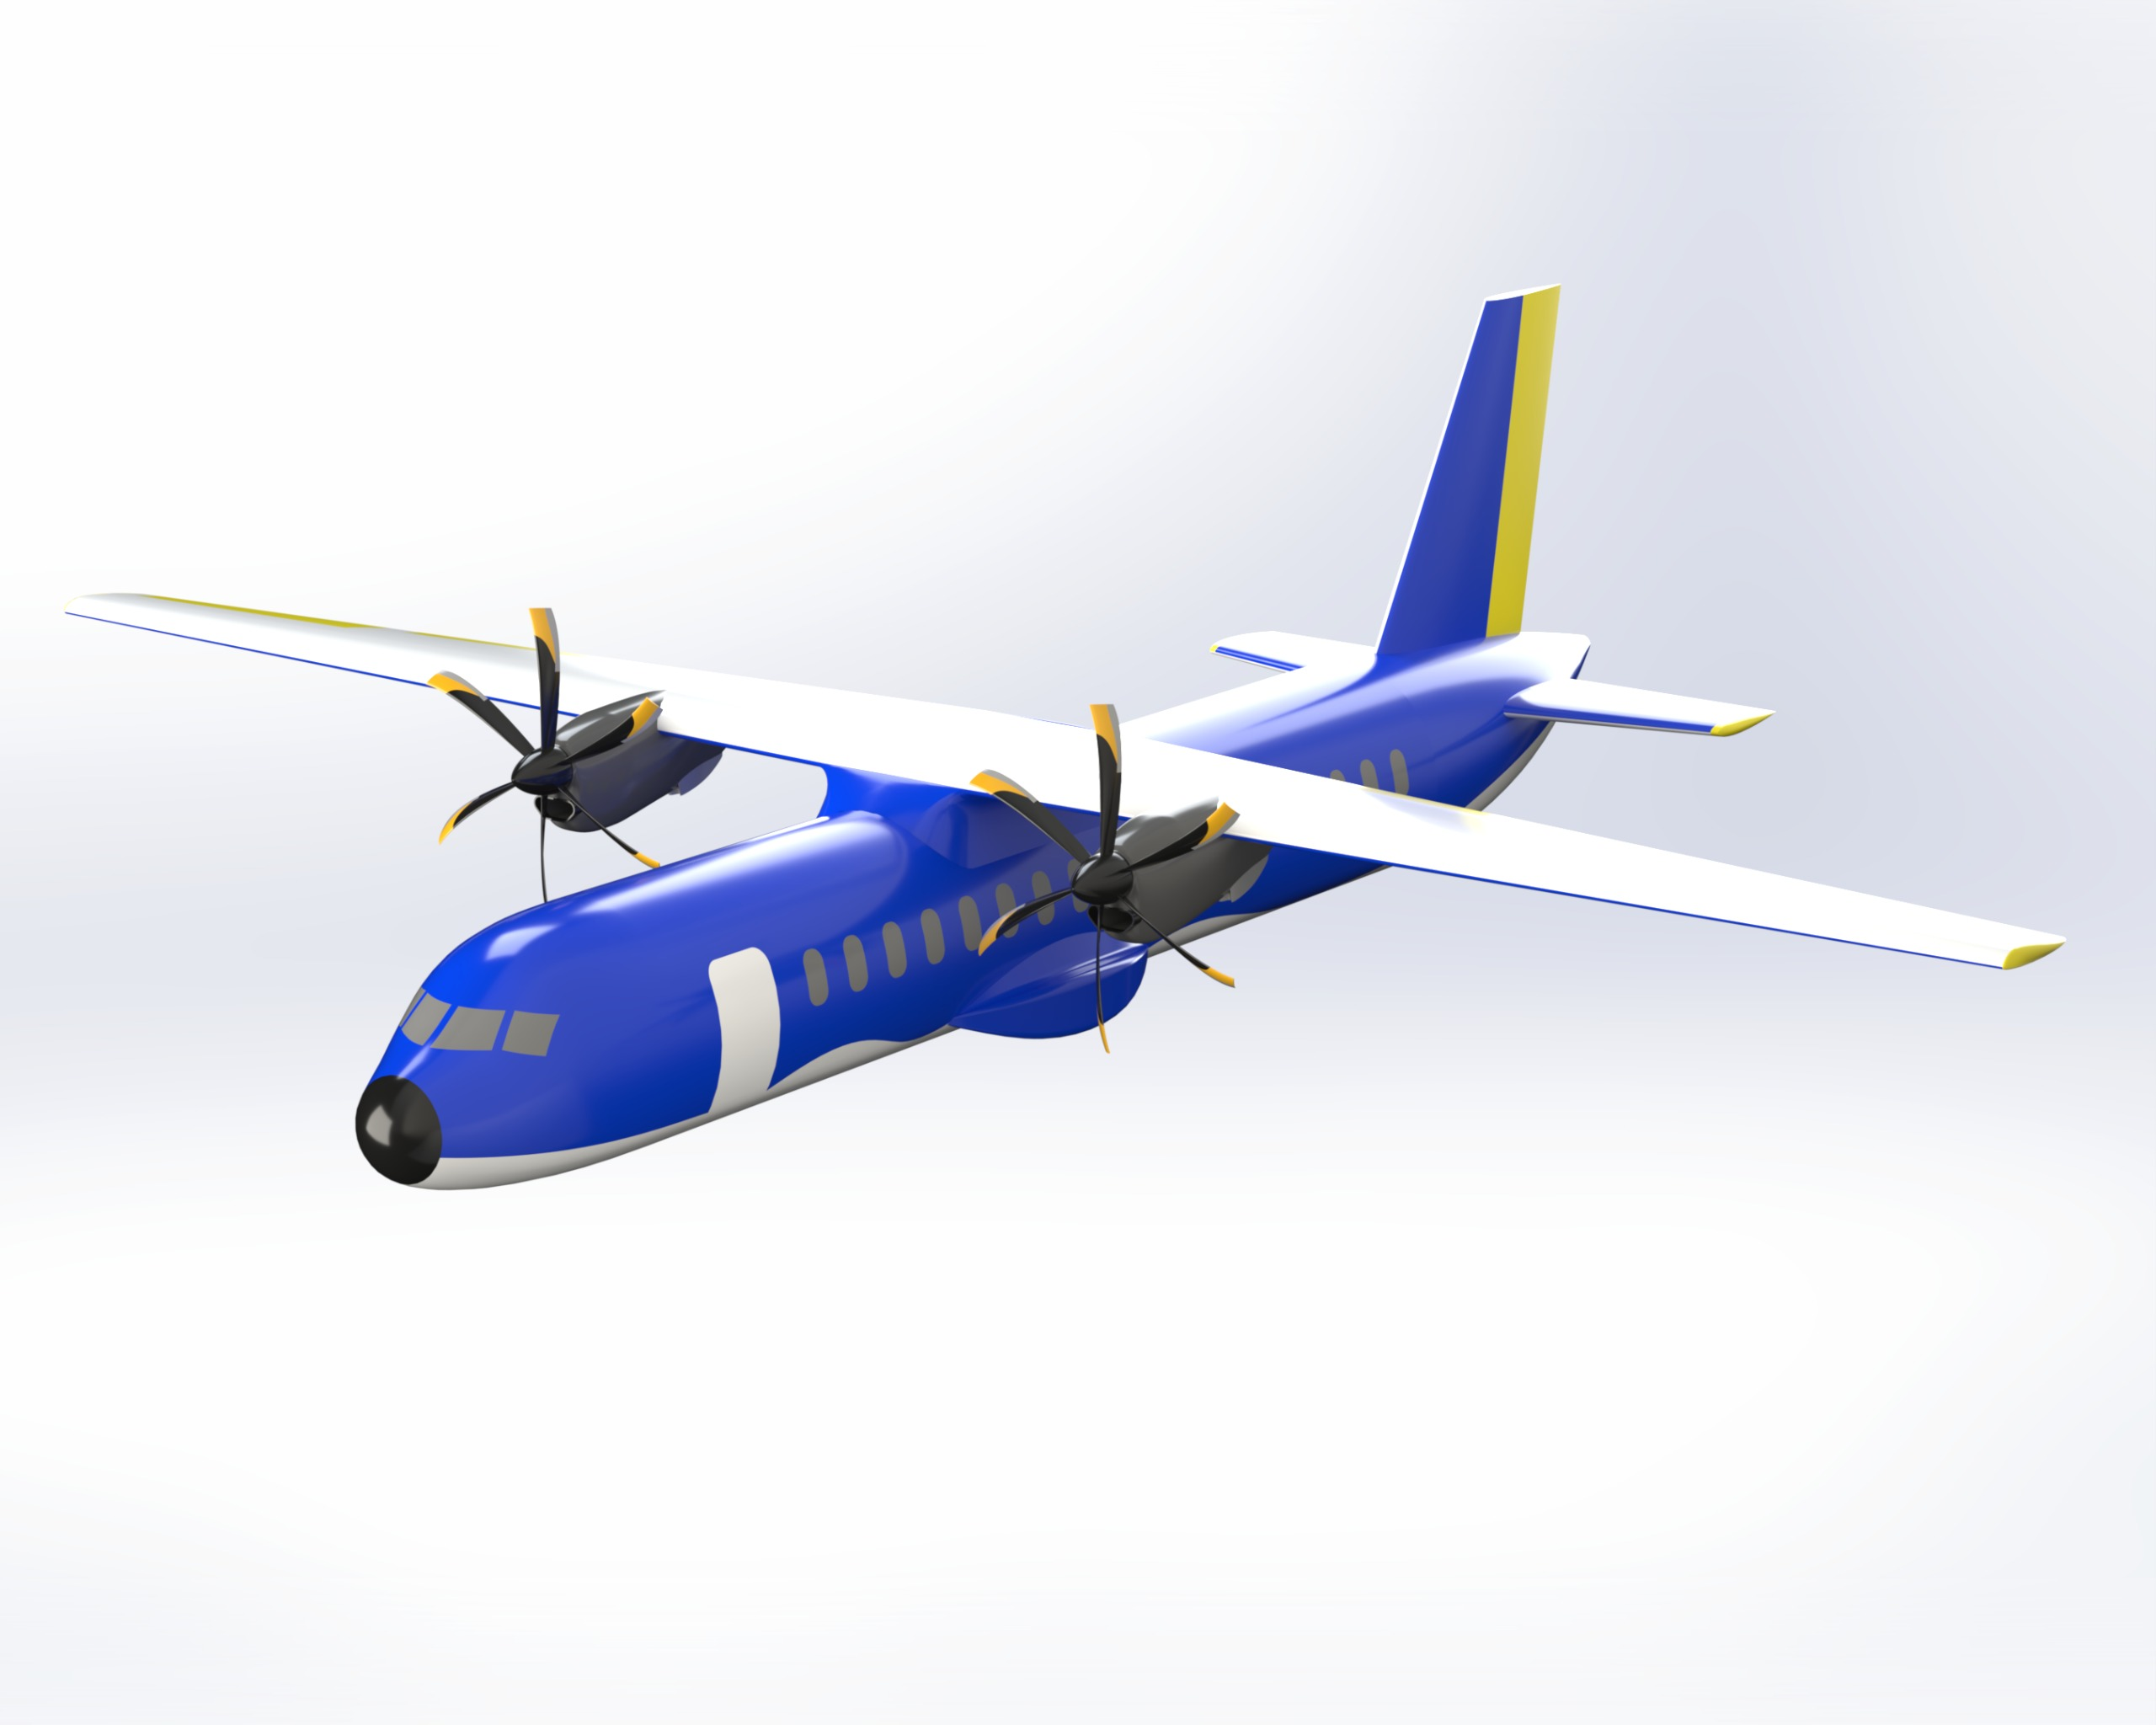
\includegraphics[width=\linewidth]{Images-2-EstudoConceitual/vista_isometrica.png}
        \caption{Vista isométrica preliminar apresentando a configuração geral e livery inicial.}
        \label{fig:vista_isometrica}
    \end{minipage}
\end{figure}